\chapter{Approach}
\label{chap:approach}
Our goal is to understand whether certain properties that we expect to be relevant for ranking can be decoded from the hidden representations of a pre-trained transformer model. Additionally, we want to know to which degree these properties are encoded at different layers within the model.

To test this, we conduct the following experiment: First, we generate a set of datasets $D_{\tx{probing}}=\{D_1, D_2, \dots, D_n \}$, each aimed at predicting a property $Y_i$ that, based on traditional ranking methods, can be considered relevant for ranking. Then, for each dataset, we train a probing classifier $P_i: \R^d \rightarrow \R^c$ on top of the fixed hidden representations $H\lay k = \{h_i\}_{i=1}^N \in \R^{N \times d}$ of subject model $\MSubject$. This procedure is repeated at every layer $k$. Finally, we compare the classifier's performance (\Cref{sec:metrics}) across layers to get a relative measure of how task-specific information is distributed throughout $\MSubject$. To better put our measurements into perspective, we also employ a random baseline model $\mathcal{B}$ which is also probed for each task separately. The probing procedure for BERT is illustrated in \Cref{fig:probing}.

Following the probing experiments, we then attempt to develop an improved fine-tuning procedure, based on our findings.

\begin{figure}[!ht]
    \centering
    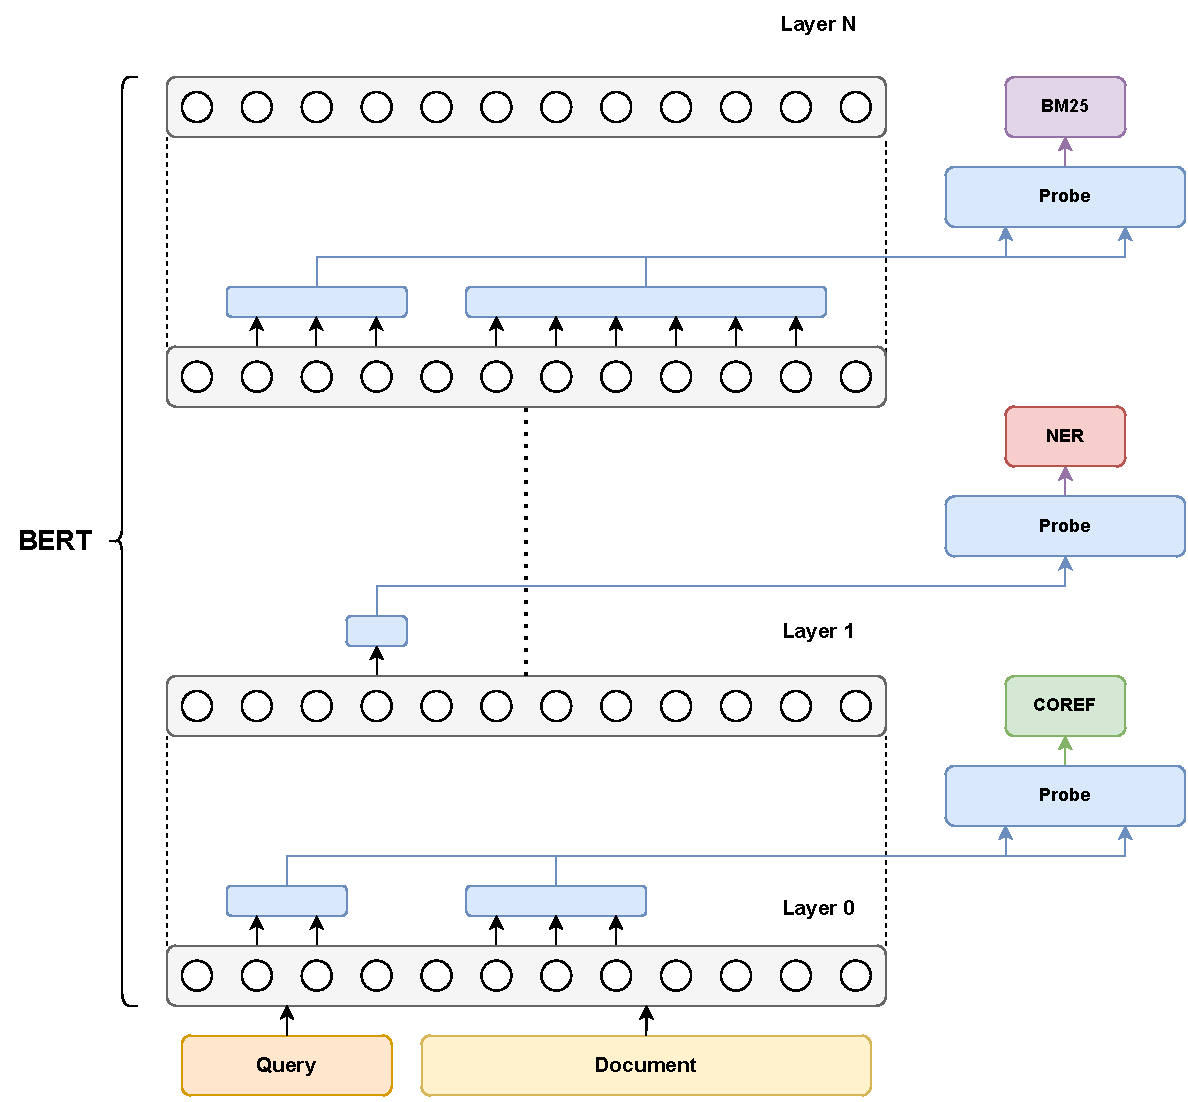
\includegraphics[width=\textwidth]{gfx/probing/probing}
    \caption{Schematic overview of the probing procedure. Each task is probed at every layer.}
    \label{fig:probing}
\end{figure}

\section{Task Design}
\label{sec:tasks}
We propose a set of classification tasks with ranking properties as target variable. \cite{tenney-etal-2019-bert} findings suggest that BERT stores language concepts in a hierarchical manner, with lower-level semantics being captured in early layers, while higher level concepts can be found closer to the output layer. To test whether this holds true for ranking, we choose tasks that require different levels of semantic abstraction in order to be solved. In this section we provide a list of the tasks we've chosen and explain the reasoning behind our selection, as well as how labels are generated automatically.

\subsubsection{BM25 Prediction}
BM25 (\Cref{sec:bm25}) is a well-known text-retrieval method and still considered a first choice when it comes to computational efficiency. As a heuristic designed around exact term matching, BM25 compares query and document on a symbolic level, without the notion of higher level semantics. Being able to decode BM25 from BERT embeddings might give a hint on whether exact matching properties like term-frequency or even corpus level statistics like inverted document-frequency are encoded by the neural ranking models.

To generate BM25 scores for each query-document pair we use the Elasticsearch BM25 implementation\footnote{\url{https://www.elastic.co/de/elasticsearch/}}.

\subsubsection{Semantic Similarity}
To measure semantic similarity, we compute cosine distance between query and document vectors in the GloVe\cite{pennington2014glove} embedding space:
\begin{equation}
    \label{eq:sem_sim}
    \tx{Sim}(q, d) = \frac{q^\top d}{||q|| \times ||d||}
\end{equation}
While these dense word representations encode semantics, unlike BERT they are not contextualized, meaning they do not change based on surrounding words in a sentence. In that sense, using semantic similarity as ranking measure may be interpreted as a kind of soft term-matching: Words between query and document that are similar in meaning increase the estimated relevance.

In order to be able to compute semantic similarity between query and document, we first embed all words in the GloVe \cite{pennington2014glove} vector space, then compute the average embedding for query and document over the sequence dimension and compare the resulting two vectors.

\subsubsection{Coreference Resolution}
Coreference resolution is the task of deciding whether two mentions in a text refer to the same entity. To model coreference we use binary classification over two spans of text in query and document, respectively.

We argue that recognizing whether an entity is shared between query and document can be an important indicator on whether the document is relevant. For instance, knowing that "the US president" in a query refers to "Joe Biden" in a document is certainly helpful.

To detect and score entity pairs, we use the neuralcoref pipeline extension for spaCy\footnote{\url{https://github.com/huggingface/neuralcoref}}. It consists of a rule-based mentions-detection module, followed by a feed-forward neural network which produces a binary coreference score for each detected pair.

\subsubsection{Named Entity Recognition}
Similar to coreference resolution, recognizing entities can be used to match concepts between query and document when performing retrieval. However, in the case of named entity recognition this matching is less restricted, as only entity \ti{types} are considered instead of specific entities. For example, given the query: "How much HP does a jaguar have?", a document that contains car entities should be prioritized over one with animal entities.

For our task, we solely test the general ability of the model to encode entities, meaning we treat document and query as a whole and predict entity types of separate text spans.

To identify named entities we use spaCy's \cite{spacy2} named entity recognition module. It is capable of detecting and assigning one of $18$ different types of entities. Naturally, we only include pairs that contain at least one entity.

\subsubsection{Fact Checking}
For fact checking, we leverage the existing FEVER \cite{thorne-etal-2018-fever} dataset. Here, instead of query and document, a claim and evidence text are provided. The goal is to classify whether the evidence supports or refutes the claim. This task requires high level semantic reasoning, making it relevant for more fine-grained ranking, i.e. providing documents that contain \ti{coherent} answers to a query and not only similar ones.

Since this is the only dataset that we don't sample from TREC2019, we can simply leverage the existing labels of FEVER and sample claim-evidence pairs from its train set.

\subsection{Probing Models}
\subsubsection{Subject Models}
\label{sec:subjects}
Subject of our probing experiments is the pre-trained BERT~\cite{devlin-etal-2019-bert} transformer model. In particular, we use the \ti{bert-base-uncased}\footnote{\url{https://huggingface.co/bert-base-uncased}} variant, which consists of $12$ layers, with $h=12$ attention heads each and a hidden dimension of $d=786$. The model has been trained on BooksCorpus~\cite{7410368} and text passages from English Wikipedia\footnote{\url{https://en.m.wikipedia.org/}}, which consist of 800 million and 2.5 billion words, respectively.

In addition, we probe two fine-tuned \ti{bert-base-uncased} models that we term \ti{bert-msm-passage} and \ti{bert-msm-doc}. Both are trained on datasets from the TREC2019 deep learning track~\cite{DBLP:journals/corr/abs-2003-07820}. While \ti{bert-msm-passage} is trained to predict relevancy of \ti{passages} given a query, \ti{bert-msm-doc} is trained on \ti{document}-level data. Thus, for this purpose we use the TREC2019 passage- and document-level dataset respectively.

Note that all three models share the same architecture and only differ by which datasets they were trained on. Having access to additional versions of \ti{bert-base-uncased} that were fine-tuned specifically for ranking, gives us a way to compare if and how the distribution of information throughout the model changes when being adapted to the new task.

Finally, as a baseline model, we probe \ti{random-embeddings}. For this we take a BERT embedding matrix and initialize its weights from a normal distribution $\sim \mathcal{N}(0, 1)$ and fix it during probing.

\subsubsection{Probe}
\label{sec:probe}
One problem in probing arises when trying to choose a probe of appropriate complexity \cite{hewitt-liang-2019-designing}. If the classifier is too complex, it might end up modeling new, complex features itself and hence, rely less on the information that is already present in the subject model's representations. On the other hand, if the classifier is too simple, it might not be able to properly decode the information at all.

While there has recently been debate on whether more complex models are actually problematic for probing \cite{pimentel-etal-2020-information}, following previous literature \cite{Tenney2019WhatDY,tenney-etal-2019-bert, hewitt-liang-2019-designing} we've decided on a simple $2$-layer MLP which, despite its simplicity, is still capable of modeling non-linear relationships.
Specifically, we use the same MLP as \cite{Tenney2019WhatDY}:

\begin{equation}
    \hat{P}(x) = \tx{LayerNorm}(\tx{tanh}(x W^{(0)} + b^{(0)})) W\lay 1 + b^{(1)}
\end{equation}
where $W\lay 0 \in \R^{|S| d \times d}$,  $W\lay 1 \in \R^{d \times c}$ and $b\lay 0 \in \R^{d}$,  $b\lay 1 \in \R^{c}$ are learned parameters with hidden size $d$ and number of target classes $c$.

Since some tasks require operating over one or multiple spans $S=\{(\tx{start}_i, {end}_i)\}_{i=1}^{|S|}$, we further need to use a pooling mechanism, such that a fixed-length representation can be provided to the probe.
Again, like \cite{Tenney2019WhatDY} we employ the simple attention pooling operator also used in \cite{lee-etal-2017-end, lee-etal-2018-higher}:

\begin{equation}
    \begin{aligned}
         & \alpha_n = \frac{\exp(w^\top h_n)}{\sum_{k=i}^j{\exp(w^\top h_k)}}   \\
         & \tx{pool}(h_i, h_{i+1},\dots, h_j)= \sum_{k=i}^j\alpha_k (W h_k + b)
    \end{aligned}
\end{equation}
where $w \in \R^{d}$, $W \in \R^{d \times d_{probe}}$, $b \in \R^{d_{probe}}$ are learned parameters which, in the case of multiple spans, are not shared between spans. The pooled span representations are concatenated and passed to the MLP, resulting in the full probe:
\begin{equation}
    P(h_1,\dots, h_N) = \hat{P}\bigg(\bigparallel_{(i, j) \in S}{\tx{pool}(h_i, h_{i+1},\dots, h_j)}\bigg)
\end{equation}

\section{Probing Setup}
\label{sec:probing_setup}
\subsection{Fine-tuning Subject Models}
We fine-tune a \ti{bert-base-uncased} model on both, TREC2019 passage- and document-level datasets (\Cref{sec:trec2019}), to obtain ranking subject models \ti{bert-msm-passage} and \ti{bert-msm-doc} (\Cref{sec:subjects}), respectively. Each model is trained with a binary cross-entropy objective, for a maximum of $20$ epochs. Early stopping is performed after $3$ epochs, if no increase in validation MAP is observed. For hyperparameters, we keep the default settings suggested by \cite{devlin-etal-2019-bert}, using the Adam optimizer\cite{kingma2014adam} with a learning rate of 1e-5, a mini-batch size of $16$ and linear increase in learning rate over the first $1000$ steps. As BERT uses a fixed set of learned positional embeddings, the input length is limited to $512$ tokens. Therefore, we truncate any passages and documents exceeding this maximum length, after applying BERT's word-piece tokenization \cite{Wu2016GooglesNM}.

\subsection{Probe Training}
All three subject models (\Cref{sec:subjects}) are probed at their intermediate output representations, meaning a classifier is learned for each layer separately. This includes the initial sequence of non-contextualized embeddings from the input embedding-matrix, which we refer to as layer $0$. We repeat this procedure for all of our proposed tasks (\Cref{sec:tasks}).

As objective function, all probing tasks use cross-entropy loss (\Cref{eq:ce_loss}) which is necessary to compute MDL. In order to achieve this, we cast regression tasks to classification tasks by binning them into $k=10$ categories. To reduce the influence of outliers, we truncate any values that are further than two standard deviations away from the mean. This means any value $< \mu - 2 \sigma$ will be assigned to class $1$ and $> \mu + 2 \sigma$ to class $10$.

We employ the Adam optimization algorithm \cite{kingma2014adam} with a learning rate of 1e-4 and a batch size of $32$ for updating the probe's parameters, while the subject model's parameters remain fixed. Learning rate is halved each epoch if the validation loss does not improve. The maximum number of epochs is set to $50$, and we stop early if validation loss has not improved in $10$ epochs. We set the probe classifier's hidden size to $d_{probe}=256$ and apply dropout with rate $0.3$ before the output layer.

All probing experiments are conducted on a server with 128GB of system memory, using a single Nvidia GTX 1080ti GPU.

\section{Evaluation Measures}
\label{sec:metrics}
In the following, we explain the evaluation measures that we employ for probing and any subsequent experiment.

\subsection{MDL}
As mentioned in \Cref{sec:probe}, selecting a proper size for a probe can be difficult. With a large probing classifier it becomes unclear whether the property probed for is decoded, or the classifier simply learns the task at hand. One way to address this problem is to compare how well the classifier performs on randomly initialized baseline representations \cite{zhang-bowman-2018-language}. Further, \cite{DBLP:journals/corr/abs-1909-03368} propose the use of \ti{control tasks}, for which task labels are randomly assigned, and a probe is selected based on the difference in accuracy to the original task. Both approaches, however, often do not reflect a large difference in accuracy when compared to the original representations or task.

As a solution, instead of accuracy, \cite{voita-titov-2020-information} propose an information theoretic approach for measuring probe performance. By recasting learning a probe model to transmitting label data with the least amount of bits, a new measure can be applied: The \ti{minimum description length} (MDL) required for transmitting the task labels, given the probed representations. Not only does MDL measure the probe's predictive performance, it also takes into account the amount of effort that is requierd for achieving said performance. The effort can manifest in model size or the amount of required training data.

Since \cite{voita-titov-2020-information} find that MDL is a more representative and also reliable measure than accuracy, we also choose it as preferred method for measuring probe performance. To compute MDL, we use the online code definition \cite{Rissanen1984UniversalCI}.
For this, the probing dataset $D=\{(x_i, y_i)\}_{i=1}^n$ is divided into timesteps $1=t_0 < t_1 < \ldots < t_S = n$. After encoding block $t_0$ with a uniform code, for each following timestep a probing model $P_{\theta_i}$ is trained on the samples $(1, \ldots, t_i)$ and used to predict over data points $(t_i + 1,\ldots, t_{i + 1})$. The full MDL is then computed as sum over the codelengths of each $P_{\theta_i}$ and the uniform encoding of the first block:

\begin{equation}
    \begin{aligned}
         & \tx{MDL}(y_{1:n} | x_{1:n}) = t_1 \log_2 c                                        \\
         & - \sum_{i=1}^{S-1} \log_2 P_{\theta_i}(y_{t_i + 1:t_{i+1}} | x_{t_i + 1:t_{i+1}})
    \end{aligned}
\end{equation}
where $c$ is the number of target classes.
Following \cite{voita-titov-2020-information}, we choose timesteps at $0.1$, $0.2$, $0.4$, $0.8$, $1.6$, $3.2$, $6.25$, $12.5$, $25$, $50$ and $100$ percent of the dataset.

\subsection{Compression}
Because it depends on the number of targets in a probing dataset, it is not reasonable to directly compare MDL between different tasks. A common way to turn MDL into a relative measure is to compute \ti{compression}. Compression divides the codelength that would result from a uniform encoding by the actual MDL:

\begin{equation}
    \tx{compression} = \frac{n \log_2(c)}{\tx{MDL}(y_{1:n} | x_{1:n})}
\end{equation}
This means compression is a measure of how much easier it is for the probe to decode a property from the probed representations, or in other words how well they encode the task labels.

\subsection{Accuracy}
As a secondary measure for probing, we further employ accuracy:
\begin{equation}
    \tx{Accuracy}(\hat{y}, y) = \frac{1}{n} \sum_{i=1}^n \mathbf{1} [\hat{y}_i = y_i]
\end{equation}
This is simply the percentage of predictions $\hat{y}$ that match the correct target $y$.

\subsection{Ranking}
Typically, ranking metrics require a set of queries $Q=\{q_i\}_{i=1}^{|Q|}$, with each query being associated with a list of labeled candidate documents $C=\{c_i\}_{i=1}^{|C|}$. The list of candidate documents is expected to be ordered in terms of their predicted relevance and each document has a ground truth label with respect to the query.

\subsubsection{MRR}
Mean reciprocal rank measures the inverse position at which the first relevant document occurs in the result set, averaged over all queries:
\begin{equation}
    \text{MRR}(Q, C) = \frac{1}{|Q|} \sum_{q \in Q} \frac{1}{\tx{rank}(q, C)}
\end{equation}
Here, $\tx{rank}(q, C)$ refers to the rank, i.e. the position of the first document in $C$ that is labeled as relevant.

\subsubsection{Precision@k}
Precision@k measures precision at a specific threshhold in $C$, i.e. only the top-$k$ results are considered when computing precision:
\begin{equation}
    \tx{Precision@}k = \bigg(\frac{\tx{\#true positives}}{\tx{\#true positives} + \tx{\#false positives}}\bigg)_k
\end{equation}

\subsubsection{MAP}
Unlike MRR, mean average precision (MAP) considers the rank of all relevant documents in the candidate set, not just the first one. Initially, average precision (AP) is computed over the set of candidates for a query:

\begin{equation}
    \text{AP}(q, C) = \frac{1}{|C_{rel}|} \sum_{k=1}^{|C|} \tx{Precision@k} \times y_k
\end{equation}
where $|C_{rel}|$ is the total number of documents marked as relevant w.r.t. the query and $y_k$ is the ground truth relevance at position $k$ in $C$. Then taking the average AP over all queries gives us MAP:

\begin{equation}
    \text{MAP}(Q, C) = \frac{1}{|Q|} \sum_{q \in Q} \text{AP}(q, C)
\end{equation}
While MRR indicates the quality of the top-ranked document, MAP provides a better picture of the full candidate set ranking.

\subsubsection{NDCG}
Normalized Discounted Cumulative Gain (NDCG) quantifies a ranked list relative to its ideal ranking. NDCG can also be applied to non-binary labels. At first, a gain is computed, that rewards early placement of relevant documents in $C$, by logarithmically scaling relevance label $y_i$ as a function of the position and summing over all labels:
\begin{equation}
    \tx{DCG} = \sum_{i=1}^{|D|} \frac{y_i}{\log_2(i+1)}
\end{equation}
Then, the ideal DCG is computed by sorting $C$ according to the ground truth labels and using it to scale DCG.
\begin{equation}
    \tx{NDCG} = \frac{\tx{DCG}}{\tx{IDCG}}
\end{equation}
This way, a perfect ordering (of which multiple may exist) will result in an NDCG of $1$ while any suboptimal ordering will lie in $[0, 1)$. Because of the logarithmic scaling, more importance is attributed to relevant documents early in the list.

